\documentclass{article}
\usepackage{tikz,pgfplots,geometry}
\pgfplotsset{compat=newest}
\usepackage[version=3]{mhchem}
\geometry{
paperwidth=15cm,paperheight=7cm,
left=0pt,right=0pt,top=1pt,bottom=0pt}
\begin{document}
\centering
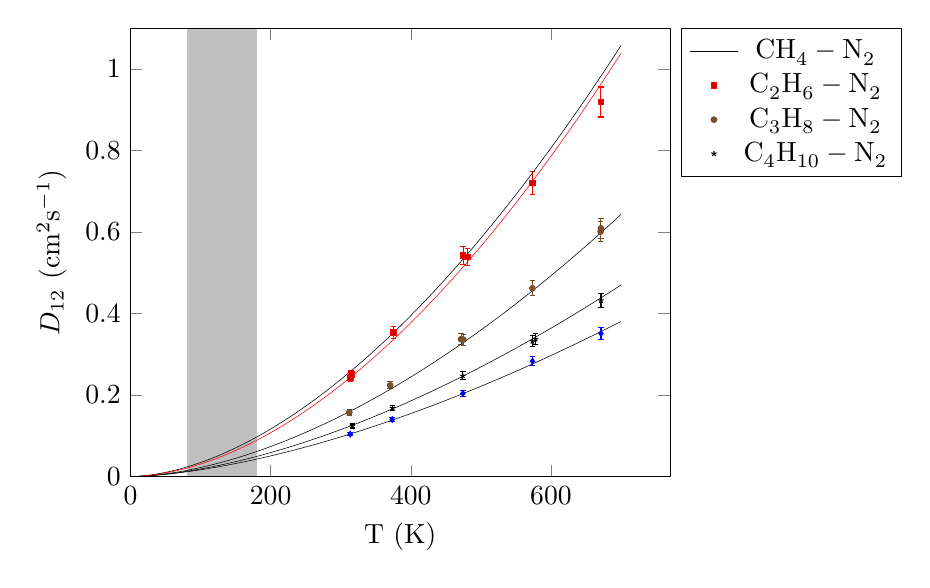
\begin{tikzpicture}
\begin{axis}[name = graph,
                xlabel = T (K),
                ylabel = $D_{12}$ (cm$^2$s$^{-1}$),
                axis on top,
                ymax = 1.1, ymin=0,
                xmin = 0,
                legend style = {at = {(1.02,1.0)}, anchor = north west}]
\addplot[draw=none,fill=gray!50] coordinates {(80,1.1) (180,1.1)}\closedcycle;
\addplot+[only marks, mark size = 1pt,
                error bars/.cd,y fixed relative = 0.04,y dir = both] coordinates{
(313.7,0.242)
(314.9,0.250)
(375.2,0.353)
(474.7,0.542)
(481.0,0.539)
(573.5,0.720)
(671.1,0.919)
};
\addlegendentry{\ce{CH4 - N2}}
\addplot+[only marks, mark size = 1pt,
                error bars/.cd,y fixed relative = 0.04,y dir = both] coordinates{
(312.2,0.157)
(370.5,0.224)
(471.7,0.337)
(474.9,0.336)
(573.46,0.462)
(670.8,0.601)
(671.2,0.609)
};
\addlegendentry{\ce{C2H6 - N2}}
\addplot+[only marks, mark size = 1pt,
                error bars/.cd,y fixed relative = 0.04,y dir = both] coordinates{
(316.5,0.124)
(373.7,0.168)
(474.2,0.247)
(573.5,0.332)
(578.1,0.337)
(671.3,0.432)
};
\addlegendentry{\ce{C3H8 - N2}}
\addplot+[only marks, mark size = 1pt,
                error bars/.cd,y fixed relative = 0.04,y dir = both] coordinates{
(313.5,0.104)
(373.5,0.140)
(474.3,0.204)
(573.5,0.283)
(671.3,0.351)
};
\addlegendentry{\ce{C4H10 - N2}}
\foreach \A/\s in {1.04/1.76 , 0.77/1.73 , 0.89/1.66 , 1.00/1.61}
\addplot[black,very thin,mark=none,domain=0:700,samples=100]{\A*1e-5*x^\s};

\foreach \D in {0.1892}
\addplot[red,very thin,mark=none,domain=0:700,samples=100]{\D*(x/273.15)^1.81};
\end{axis}
\end{tikzpicture}
\end{document}
